\documentclass[aspectratio=169,11pt]{beamer}

% ── Packages ──────────────────────────────────────────────────────────────────
\usepackage{graphicx}
\usepackage{booktabs}
\usepackage{array}
\usepackage{xcolor}
\usepackage{tikz}
\usetikzlibrary{calc, positioning}
\usepackage{amsmath}
\usepackage{hyperref}
\usepackage{siunitx}
\usepackage{colortbl}

% ── Colour Palette ────────────────────────────────────────────────────────────
\definecolor{DeepNavy}{HTML}{2E4057}
\definecolor{Teal}{HTML}{048A81}
\definecolor{WarmOrange}{HTML}{E85D04}
\definecolor{SoftPurple}{HTML}{9D4EDD}
\definecolor{WarmGray}{HTML}{8A8A8A}
\definecolor{LightGray}{HTML}{F2F2F2}
\definecolor{Cream}{HTML}{FFFDF7}
\definecolor{DeepRed}{HTML}{C1121F}
\definecolor{Gold}{HTML}{D4A017}

% ── Theme Setup ───────────────────────────────────────────────────────────────
\usetheme{default}
\setbeamertemplate{navigation symbols}{}
\setbeamertemplate{headline}{}
\setbeamercolor{background canvas}{bg=Cream}
\setbeamercolor{frametitle}{fg=DeepNavy,bg=Cream}
\setbeamerfont{frametitle}{series=\bfseries,size=\large}

\setbeamertemplate{frametitle}{%
  \vspace*{0.3em}%
  \insertframetitle%
  \ifx\insertframesubtitle\empty\else
    \\[0.1em]{\footnotesize\color{WarmGray}\insertframesubtitle}%
  \fi
  \vspace*{0.15em}%
  \textcolor{Teal}{\rule{\textwidth}{0.5pt}}%
}

\setbeamertemplate{footline}{%
  \hfill{\color{WarmGray}\tiny\insertframenumber\hspace{0.5em}}%
  \vspace{0.3em}%
}

\setbeamercolor{itemize item}{fg=Teal}
\setbeamercolor{itemize subitem}{fg=WarmOrange}
\setbeamertemplate{itemize item}{\small\raisebox{0.15ex}{\textbullet}}
\setbeamertemplate{itemize subitem}{\scriptsize\raisebox{0.15ex}{\textbullet}}

% ── Custom Macros ─────────────────────────────────────────────────────────────
\newcommand{\emphcolor}[1]{{\color{WarmOrange}\textbf{#1}}}
\newcommand{\tealtext}[1]{{\color{Teal}#1}}
\newcommand{\navytext}[1]{{\color{DeepNavy}#1}}
\newcommand{\graytext}[1]{{\color{WarmGray}#1}}

\newcommand{\transitionslide}[2]{%
  \begingroup
  \setbeamercolor{background canvas}{bg=DeepNavy}
  \setbeamertemplate{footline}{}
  \begin{frame}[plain]
    
\begin{tikzpicture}[overlay]
      \draw[Teal, opacity=0.3, line width=8pt]
        (-1,-1) -- ++(20,0) -- ++(0,12) -- cycle;
    \end{tikzpicture}
    \vspace{1.8cm}
    \hspace{0.8cm}%
    {\color{white}\bfseries\LARGE\parbox{13cm}{#1}}\\[0.6em]
    \hspace{0.8cm}%
    {\color{Teal}\normalsize\parbox{13cm}{#2}}
  \end{frame}%
  \endgroup
}

% ── Document ──────────────────────────────────────────────────────────────────
\begin{document}

% ── Slide 1: Title ────────────────────────────────────────────────────────────
\begingroup
\setbeamercolor{background canvas}{bg=DeepNavy}
\setbeamertemplate{footline}{}
\begin{frame}[plain]
  \begin{tikzpicture}[overlay]
    \node[text=Teal, opacity=0.12, font=\fontsize{140}{140}\selectfont]
      at (10, 2.5) {\(\sim\)};
  \end{tikzpicture}
  \vspace{0.9cm}
  \hspace{0.6cm}%
  {\color{white}\bfseries\fontsize{22}{28}\selectfont
    \parbox{13cm}{Climate Shocks, Health Finance,\\and Economic Outcomes}}
  \par\vspace{0.45em}
  \hspace{0.6cm}%
  {\color{WarmOrange}\rule{12cm}{2pt}}
  \par\vspace{0.45em}
  \hspace{0.6cm}%
  {\color{Teal}\normalsize County-Level Evidence from the United States, 2011--2023}
  \par\vspace{0.35em}
  \hspace{0.6cm}%
  {\color{WarmGray}\small Thesis Committee Update \(\cdot\) March 2026}
\end{frame}
\endgroup

% ── Slide 2: Transition — State ───────────────────────────────────────────────
\transitionslide{State-Level Results}{Two-way FE: State + Year,\ \ N\(\approx\)550--650,\ \ cluster = State}

% ── Slide 3: State — Key Significant Findings ────────────────────────────────
\begin{frame}{State-Level: Key Significant Results}
  \framesubtitle{Two-way FE (State + Year), state-clustered SEs; $^{*}p{<}0.10$, $^{**}p{<}0.05$, $^{***}p{<}0.01$}
  \small
  \begin{columns}[T]
    \begin{column}{0.50\textwidth}
      \textbf{\tealtext{Employer Premiums} (\$2025)}\\[0.3em]
      \begin{tabular}{lrl}
        \toprule
        Predictor & Coef. & \\
        \midrule
        Extreme Drought ($h{=}0$) & $+63.6$ & \emphcolor{**} \\
        Severe Drought ($h{=}0$) & $+86.4$ & \emphcolor{***} \\
        Severe Drought (lag 1) & $+65.1$ & \emphcolor{**} \\
        Pct PM$_{2.5}$ days & $+20.8$ & \emphcolor{***} \\
        Pct PM$_{10}$ days & $+22.7$ & \emphcolor{***} \\
        Pct Ozone days & $+19.7$ & \emphcolor{***} \\
        \bottomrule
      \end{tabular}
      \vspace{0.5em}

      \textbf{\tealtext{Medical Debt Share (pp)}}\\[0.3em]
      \begin{tabular}{lrl}
        \toprule
        Predictor & Coef. & \\
        \midrule
        Cold Shock (lag 1) & $+0.0135$ & \emphcolor{**} \\
        \bottomrule
      \end{tabular}
    \end{column}
    \begin{column}{0.46\textwidth}
      \textbf{\tealtext{Medical Debt Median (\$2025)}}\\[0.3em]
      \begin{tabular}{lrl}
        \toprule
        Predictor & Coef. & \\
        \midrule
        High HDD ($h{=}0$) & $+58.9$ & \emphcolor{**} \\
        Severe Drought ($h{=}0$) & $-66.8$ & \emphcolor{***} \\
        Severe Drought (lag 1) & $-37.5$ & \emphcolor{**} \\
        \bottomrule
      \end{tabular}
      \vspace{0.5em}

      \textbf{\tealtext{Medicare per Enrollee (\$)}}\\[0.3em]
      \begin{tabular}{lrl}
        \toprule
        Predictor & Coef. & \\
        \midrule
        High CDD (lag 1) & $+144.7$ & \emphcolor{**} \\
        High CDD (lag 2) & $+137.2$ & \emphcolor{***} \\
        High HDD (lag 1) & $-110.1$ & \emphcolor{*} \\
        High HDD (lag 2) & $-192.7$ & \emphcolor{***} \\
        \bottomrule
      \end{tabular}
      \vspace{0.3em}

      \graytext{\scriptsize Cold Shock $\to$ Total Health Exp: $+\$205.3^{**}$\quad
      Severe Drought $\to$ Medicaid/Enrollee: $-\$524.5^{***}$}
    \end{column}
  \end{columns}
\end{frame}

% ── Slide 4: State — Cold vs. Heat Asymmetry ─────────────────────────────────
\begin{frame}{State-Level: Cold and Heat Have Opposite Channels}
  \framesubtitle{State-level FE; March 2026}
  \begin{columns}[T]
    \begin{column}{0.56\textwidth}
      \begin{center}
      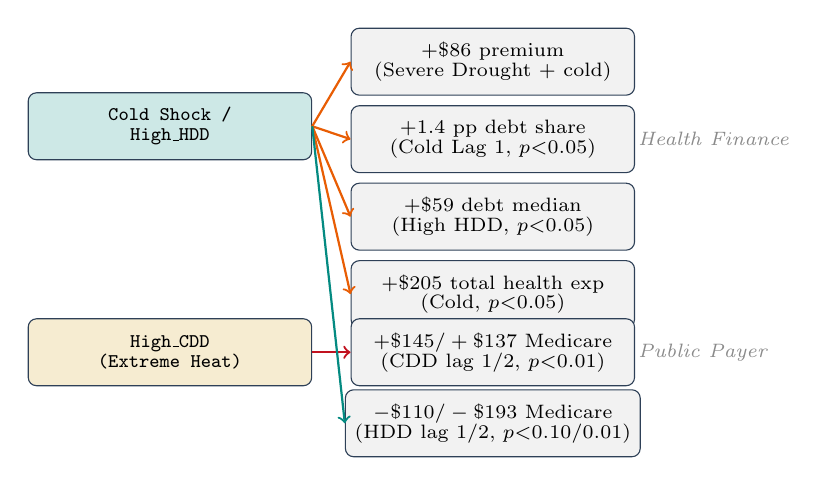
\begin{tikzpicture}[scale=0.82,
        box/.style={draw=DeepNavy, rounded corners=3pt, fill=LightGray,
                    minimum width=3.6cm, minimum height=0.85cm, align=center, font=\scriptsize}]

        \node[box, fill=Teal!20] (cold) at (0,0)   {\texttt{Cold Shock /}\\[-0.1em]\texttt{High\_HDD}};
        \node[box, fill=Gold!20] (heat) at (0,-3.5) {\texttt{High\_CDD}\\[-0.1em]\texttt{(Extreme Heat)}};

        \node[box] (prem)  at (5.0, 1.0)  {$+\$86$ premium\\[-0.1em](Severe Drought $+$ cold)};
        \node[box] (debt)  at (5.0,-0.2)  {$+1.4$ pp debt share\\[-0.1em](Cold Lag 1, $p{<}0.05$)};
        \node[box] (med)   at (5.0,-1.4)  {$+\$59$ debt median\\[-0.1em](High HDD, $p{<}0.05$)};
        \node[box] (exp)   at (5.0,-2.6)  {$+\$205$ total health exp\\[-0.1em](Cold, $p{<}0.05$)};
        \node[box] (mcare1) at (5.0,-3.5) {$+\$145/+\$137$ Medicare\\[-0.1em](CDD lag 1/2, $p{<}0.01$)};
        \node[box] (mcare2) at (5.0,-4.6) {$-\$110/-\$193$ Medicare\\[-0.1em](HDD lag 1/2, $p{<}0.10/0.01$)};

        \draw[->, WarmOrange, thick] (cold.east) -- (prem.west);
        \draw[->, WarmOrange, thick] (cold.east) -- (debt.west);
        \draw[->, WarmOrange, thick] (cold.east) -- (med.west);
        \draw[->, WarmOrange, thick] (cold.east) -- (exp.west);
        \draw[->, DeepRed, thick]    (heat.east) -- (mcare1.west);
        \draw[->, Teal, thick]       (cold.east) -- (mcare2.west);

        \node[font=\scriptsize\itshape, text=WarmGray, anchor=west] at (7.1,-0.2)  {Health Finance};
        \node[font=\scriptsize\itshape, text=WarmGray, anchor=west] at (7.1,-3.5) {Public Payer};
      \end{tikzpicture}
      \end{center}
    \end{column}
    \begin{column}{0.40\textwidth}
      \small
      \textbf{Cold channel:}
      \begin{itemize}\itemsep0.2em
        \item Raises premiums via drought co-occurrence
        \item Lagged debt accumulation
        \item Boosts total system expenditure
      \end{itemize}
      \vspace{0.4em}
      \textbf{Heat channel (CDD):}
      \begin{itemize}\itemsep0.2em
        \item Raises Medicare spending with 1--2 year lag
        \item Consistent with elderly heat-related utilisation
      \end{itemize}
      \vspace{0.4em}
      \textbf{Cold channel (HDD):}
      \begin{itemize}\itemsep0.2em
        \item Reduces Medicare with 1--2 year lag
        \item Possible substitution or coding effects
      \end{itemize}
      \vspace{0.4em}
      \tealtext{\footnotesize Novel finding: heat and cold affect public payers\\in opposite directions.}
    \end{column}
  \end{columns}
\end{frame}

% ── Slide 5: Transition — County ──────────────────────────────────────────────
\transitionslide{County-Level Results}{Two-way FE: County + Year,\ \ N\(\approx\)23k--34k,\ \ cluster = State}

% ── Slide 6: County — Medical Debt ───────────────────────────────────────────
\begin{frame}{County: Heat Raises Debt Severity; Cold Raises Debt Prevalence}
  \framesubtitle{Outcomes: Medical Debt Share (pp) and Median Debt (\$2023); state-clustered SEs}
  \small
  \begin{columns}[T]
    \begin{column}{0.47\textwidth}
      \tealtext{\textbf{Z\_Temp (Relative Heat)}}\\[0.3em]
      \begin{tabular}{lccc}
        \toprule
        & UW & PW & \\
        \midrule
        \multicolumn{4}{l}{\textit{Debt Share (pp)}} \\
        $h{=}0$  & $-0.0025$ & $-0.0000$ & \\
        Lag 2    & \emphcolor{$-0.0027^{**}$} & \emphcolor{$-0.0014^{*}$} & \\
        \midrule
        \multicolumn{4}{l}{\textit{Debt Median (\$)}} \\
        $h{=}0$  & \emphcolor{$+14.9^{*}$} & \emphcolor{$+18.5^{***}$} & \\
        Lag 2    & \emphcolor{$+19.5^{**}$} & \emphcolor{$+16.2^{***}$} & \\
        \bottomrule
      \end{tabular}
      \vspace{0.4em}
      \graytext{\scriptsize UW = unweighted; PW = pop-weighted.}\\[0.2em]
      \graytext{\scriptsize Pattern: heat reduces share (protective?) but\\raises median severity — composition effect.}
    \end{column}
    \begin{column}{0.47\textwidth}
      \tealtext{\textbf{High\_HDD (Extreme Cold Burden)}}\\[0.3em]
      \begin{tabular}{lccc}
        \toprule
        & UW & PW & \\
        \midrule
        \multicolumn{4}{l}{\textit{Debt Share (pp)}} \\
        $h{=}0$  & \emphcolor{$+0.0038^{**}$} & \emphcolor{$+0.0054^{**}$} & \\
        Lag 2    & $+0.0031^{*}$ & $+0.0037^{*}$ & \\
        \midrule
        \multicolumn{4}{l}{\textit{Debt Median (\$)}} \\
        $h{=}0$  & $+10.6$ & \emphcolor{$+31.2^{**}$} & \\
        \bottomrule
      \end{tabular}
      \vspace{0.4em}
      \textbf{Controls (both outcomes):}\\
      \begin{tabular}{lr}
        Uninsured Rate & \emphcolor{$+^{***}$ (large)} \\
        HH Income & \emphcolor{$-^{**}$} \\
      \end{tabular}
    \end{column}
  \end{columns}
\end{frame}

% ── Slide 7: County — Insurance Premiums ──────────────────────────────────────
\begin{frame}{County: Cold Dominates Premium Signal; Heat Effect is Lagged}
  \framesubtitle{Outcome: Benchmark Silver Premium (\$2023 real); county FE + Year FE}
  \small
  \begin{columns}[T]
    \begin{column}{0.47\textwidth}
      \tealtext{\textbf{High\_HDD — Cold Burden}}\\[0.25em]
      \begin{tabular}{lrrl}
        \toprule
        Spec & UW & PW & Cluster \\
        \midrule
        $h{=}0$ & \emphcolor{$+28.1^{***}$} & \emphcolor{$+21.9^{**}$} & State \\
        $h{=}0$ & \emphcolor{$+28.1^{***}$} & \emphcolor{$+21.9^{***}$} & RA \\
        Lag 1   & $-24.5^{*}$ & $-20.8$ & State \\
        \bottomrule
      \end{tabular}
      \vspace{0.5em}

      \tealtext{\textbf{High\_CDD — Heat Burden (lag)}}\\[0.25em]
      \begin{tabular}{lrrl}
        \toprule
        Spec & UW & PW & Cluster \\
        \midrule
        Lag 1 & $+8.7$ & \emphcolor{$+31.4^{***}$} & RA \\
        Lag 2 & \emphcolor{$+21.6^{*}$} & \emphcolor{$+35.3^{***}$} & RA \\
        \bottomrule
      \end{tabular}
    \end{column}
    \begin{column}{0.47\textwidth}
      \tealtext{\textbf{Z\_Temp — Relative Temperature}}\\[0.25em]
      \begin{tabular}{lrrl}
        \toprule
        Spec & UW & PW & Cluster \\
        \midrule
        $h{=}0$ & \emphcolor{$-10.9^{**}$} & $+2.7$ & RA \\
        Lag 1   & $+3.8$ & \emphcolor{$+5.4^{**}$} & RA \\
        Lag 2   & $+1.0$ & \emphcolor{$+4.2^{**}$} & RA \\
        \bottomrule
      \end{tabular}
      \vspace{0.5em}
      \begin{itemize}\itemsep0.3em
        \item \emphcolor{Cold burden contemporaneously raises premiums} across all specs
        \item Heat reduces premiums at $h{=}0$ but raises them with 1--2 year lag
        \item RA-clustering tightens SEs; results robust
        \item Drought (PDSI lag 1): $+\$3.9$ in RA spec ($p{=}0.05$)
      \end{itemize}
    \end{column}
  \end{columns}
\end{frame}

% ── Slide 8: County — Hospital Bad Debt & Income ─────────────────────────────
\begin{frame}{County: Heat Lag Reduces Hospital Bad Debt; Raises HH Income Anomaly}
  \framesubtitle{Outcomes: Hosp.\ Bad Debt per Capita (\$) and Median HH Income (\$2023)}
  \small
  \begin{columns}[T]
    \begin{column}{0.47\textwidth}
      \tealtext{\textbf{Hospital Bad Debt / Capita}}\\[0.3em]
      \begin{tabular}{lcc}
        \toprule
        Predictor & UW & PW \\
        \midrule
        Z\_Temp Lag 2 & \emphcolor{$-2.41^{***}$} & \emphcolor{$-2.08^{***}$} \\
        High\_HDD ($h{=}0$) & \emphcolor{$+5.33^{***}$} & \emphcolor{$+4.23^{**}$} \\
        PDSI Lag 1 & $+0.57^{*}$ & — \\
        Uninsured & \emphcolor{$+^{***}$} & \\
        \bottomrule
      \end{tabular}
      \vspace{0.4em}
      \graytext{\scriptsize Heat lag reduces bad debt — possible reduction\\in utilisation or elective procedure deferral.\\Cold raises bad debt contemporaneously.}
    \end{column}
    \begin{column}{0.47\textwidth}
      \tealtext{\textbf{Median HH Income (\$2023)}}\\[0.3em]
      \begin{tabular}{lcc}
        \toprule
        Predictor & UW & PW \\
        \midrule
        Z\_Temp ($h{=}0$)  & $-71^{**}$ & \emphcolor{$-88^{***}$} \\
        Z\_Temp Lag 1       & $-36$ & \emphcolor{$-64^{***}$} \\
        Z\_Temp Lag 2       & \emphcolor{$-71^{**}$} & \emphcolor{$-60^{**}$} \\
        High\_CDD ($h{=}0$) & \emphcolor{$-247^{**}$} & $-3$ \\
        High\_HDD ($h{=}0$) & $+161^{**}$ & \emphcolor{$+173^{***}$} \\
        \bottomrule
      \end{tabular}
      \vspace{0.3em}
      \graytext{\scriptsize Relative heat consistently \emphcolor{reduces} HH income.\\Cold (HDD) \emphcolor{raises} income — possible energy/agriculture mix.}
    \end{column}
  \end{columns}
\end{frame}

% ── Slide 9: County — PCPI & Employment ──────────────────────────────────────
\begin{frame}{County: Drought Depresses Income; Cold Suppresses Employment}
  \framesubtitle{Outcomes: Per Capita Personal Income (\$) and Civilian Employment (persons)}
  \small
  \begin{columns}[T]
    \begin{column}{0.47\textwidth}
      \tealtext{\textbf{Per Capita Personal Income}}\\[0.3em]
      \begin{tabular}{lcc}
        \toprule
        Predictor & UW & PW \\
        \midrule
        PDSI Lag 2  & $-8.5$ & \emphcolor{$-112.9^{**}$} \\
        High\_CDD Lag 1 & \emphcolor{$+480^{**}$} & $-116$ \\
        \multicolumn{3}{l}{\textit{RA-level robustness (pop-wtd):}} \\
        PDSI ($h{=}0$) & \multicolumn{2}{c}{\emphcolor{$-205.7^{***}$}} \\
        PDSI Lag 1      & \multicolumn{2}{c}{$-54.5$} \\
        \bottomrule
      \end{tabular}
      \vspace{0.3em}
      \graytext{\scriptsize Strong drought signal at Rating-Area level:\\$-\$206$ per capita per PDSI unit ($p{<}0.001$).}
    \end{column}
    \begin{column}{0.47\textwidth}
      \tealtext{\textbf{Civilian Employment (persons)}}\\[0.3em]
      \begin{tabular}{lcc}
        \toprule
        Predictor & UW & PW \\
        \midrule
        Z\_Temp Lag 2       & \emphcolor{$+788^{**}$} & $+3216$ \\
        High\_HDD ($h{=}0$) & \emphcolor{$-468^{**}$} & $+2587$ \\
        High\_HDD Lag 2     & \emphcolor{$-678^{**}$} & $+3988$ \\
        Z\_Precip ($h{=}0$) & $+46$ & \emphcolor{$-5742^{***}$} \\
        Z\_Precip Lag 1     & $-88$ & \emphcolor{$-3803^{***}$} \\
        \bottomrule
      \end{tabular}
      \vspace{0.3em}
      \graytext{\scriptsize Pop-weighted spec: dry conditions strongly\\reduce employment in populated counties.\\Unweighted: cold suppresses employment,\\heat lag raises it.}
    \end{column}
  \end{columns}
\end{frame}

% ── Slide 10: Transition — Synthesis ──────────────────────────────────────────
\transitionslide{Cross-Level Synthesis}{What do state and county results agree on?}

% ── Slide 11: Synthesis — Convergent Findings ────────────────────────────────
\begin{frame}{State and County Pipelines Tell a Consistent Story}
  \framesubtitle{Key findings replicated across both levels of analysis}
  \begin{center}
  \small
  \renewcommand{\arraystretch}{1.5}
  \begin{tabular}{lcc}
    \rowcolor{DeepNavy}
    \textcolor{white}{\textbf{Finding}} &
    \textcolor{white}{\textbf{State}} &
    \textcolor{white}{\textbf{County}} \\
    \rowcolor{Teal!10}
    Cold / High HDD $\to$ higher health finance costs &
    \tealtext{\textbf{\checkmark}} & \tealtext{\textbf{\checkmark}} \\
    Drought $\to$ reduced Medicaid / Medicare spending &
    \tealtext{\textbf{\checkmark}} & \tealtext{\textbf{\checkmark}} \graytext{\scriptsize(PDSI)} \\
    \rowcolor{Teal!10}
    Heat $\to$ household income loss &
    \graytext{---} & \tealtext{\textbf{\checkmark}} \graytext{\scriptsize(Z\_Temp***)} \\
    HDD $\to$ medical debt (share \& median) &
    \tealtext{\textbf{\checkmark}} \graytext{\scriptsize(Median)} &
    \tealtext{\textbf{\checkmark}} \graytext{\scriptsize(Share+Med)} \\
    \rowcolor{Teal!10}
    Poor air quality $\to$ higher premiums &
    \tealtext{\textbf{\checkmark}} \graytext{\scriptsize(PM$_{2.5}$/O$_3$***)} &
    \graytext{\scriptsize not modeled} \\
    Drought / dry conditions $\to$ employment loss &
    \graytext{---} & \tealtext{\textbf{\checkmark}} \graytext{\scriptsize(Z\_Precip***)} \\
  \end{tabular}
  \end{center}
\end{frame}

% ── Slide 12: Diagnostics & Robustness ───────────────────────────────────────
\begin{frame}{Model Diagnostics and Robustness}
  \framesubtitle{Both pipelines pass standard specification checks}
  \begin{columns}[T]
    \begin{column}{0.47\textwidth}
      \textbf{\tealtext{State-Level}}
      \begin{itemize}\itemsep0.25em
        \item $N = 550$--$650$; Within-$R^2 = 0.09$--$0.21$
        \item \texttt{Pct\_NO2} dropped by \texttt{fixest} (collinear with other AQI vars)
        \item VIF max $\approx 5.3$ after PDSI-only drought block
        \item CDD/HDD thresholds: national p80, 1990--2000 baseline (corrected from within-state all-years)
        \item \texttt{is\_high\_hdd} newly added this session
      \end{itemize}
    \end{column}
    \begin{column}{0.47\textwidth}
      \textbf{\tealtext{County-Level}}
      \begin{itemize}\itemsep0.25em
        \item $N = 23$k--$34$k; Within-$R^2$ up to $0.81$ (HH Income), $0.44$ (PCPI)
        \item Rating-Area clustered SEs: tighten confidence intervals; core results survive
        \item RA-level robustness aggregation: pop-weighted, lags re-estimated
        \item \textbf{Debt exclusion:} CO 2023 removed (HB23-1126, Aug snapshot); $60$ obs excluded
        \item Z-scores anchored to 1990--2000 per-county baseline (no look-ahead)
      \end{itemize}
    \end{column}
  \end{columns}
  \vspace{0.4em}
  \begin{center}
    \graytext{\small Full coefficient tables: \texttt{Analysis/state\_regression\_results.md} and \texttt{county\_regression\_results.md}}
  \end{center}
\end{frame}

% ── Slide 13: Next Steps ──────────────────────────────────────────────────────
\begin{frame}{Next Steps}
  \framesubtitle{Planned extensions to the empirical framework}
  \begin{columns}[T]
    \begin{column}{0.47\textwidth}
      \textbf{\tealtext{Empirical Extensions}}
      \begin{itemize}\itemsep0.35em
        \item \emphcolor{Event study / local projections:} IRFs for \texttt{High\_CDD}, \texttt{High\_HDD}, \texttt{Is\_Extreme\_Drought}, \texttt{High\_AQI\_Max} — dynamic impulse-response over $h = 0$--$4$
        \item \emphcolor{County unemployment:} BLS LAUS integration planned (currently proxied by ACS employment)
        \item \emphcolor{Mechanism decomposition:} separate cold-weather respiratory illness channel from energy-poverty channel
      \end{itemize}
    \end{column}
    \begin{column}{0.47\textwidth}
      \textbf{\tealtext{Writing and Defence}}
      \begin{itemize}\itemsep0.35em
        \item \emphcolor{Dissertation chapter draft:} integrate state and county findings into unified narrative
        \item \emphcolor{Heterogeneity analysis:} rural vs.\ urban counties; high vs.\ low baseline AQI
        \item \emphcolor{Policy counterfactuals:} ACA Medicaid expansion interaction with climate shocks
      \end{itemize}
      \vspace{0.6em}
      \tealtext{\small All pipeline code version-controlled; analysis-ready datasets documented in \texttt{CLAUDE.md}.}
    \end{column}
  \end{columns}
\end{frame}

\end{document}
